\ifdefined\isstandalone
\title{6.047/6.878 Lecture 21: Phylogenomics II {\tmabbr{}}}
\author{Guest Lecture by\\
  Matt Rasmussen \\
  Orit Giguzinsky and Ethan Sherbondy}
\maketitle
\chead{6.047/6.878 Lecture 21: Phylogenomics II}
\lhead{}
\rhead{}
{\pagebreak}
{\tableofcontents}
{\pagebreak}
{\listoffigures}
\else
\chapter{Phylogenomics II}
\author{Guest Lecture by\\
  Matt Rasmussen \\
  2012: Updated by Orit Giguzinsky and Ethan Sherbondy}
\chead{6.047/6.878 Lecture 21: Phylogenomics II}
\lhead{} 
\rhead{} 
\minilof
\fi 
\pagestyle{fancy} 

\ifdefined\isstandalone
\def\@mydir{images} 
\fi
\ifdefined\ischapter
\def\@mydir{../Lecture21_Phylogenomics/images} 
\fi 
\ifdefined\ismaster
\def\@mydir{Lecture21_Phylogenomics/images} 
\fi 
% ####################################################################
\section{Introduction}

In the previous chapter, we covered techniques for reasoning about evolution in terms of trees of descent. The algorithms we covered for tree-building, UPGMA and neighbor-joining, assumed that we were comparing fully aligned sections of sequences.

In this section, we present additional models for using phylogenetic trees in different contexts. Here we clarify the differences between species and gene trees. We then cover a framework called reconciliation which lets us effectively combine the two by mapping gene trees onto species trees. This mapping gives us a means of inferring gene duplication and loss events.

We will also present a phylogenetic perspective for reasoning about population genetics. Since population genetics deals with relatively recent mutation events, we offer the Wright-Fisher model as a tool for representing changes in whole populations. Unfortunately, when dealing with real-world data, we usually are only able to sequence genes from the current living descendants of a group. As a remedy to this shortcoming, we cover the Coalescent model, which you can think of as a time-reversed Wright-Fisher analog.

By using coalescence, we gain a new means for estimating divergence times and population sizes across multiple species. At the end of the chapter, we touch briefly on the challenges of using trees to model recombination events and summarize recent work in the field along with frontiers open for exploration.

\section{Inferring Orthologs/Paralogs, Gene Duplication and Loss}

\noindent There are two commonly used trees, Species tree and Gene tree. This section explains how these trees can be used and how to fit a gene tree inside a species tree (reconciliation).

\subsection {Species Tree}
Species trees that show how different species evolved from one another. These trees are created using morphological characters, fossil evidence, etc. The leaves of each tree are labeled as species and the rest of the tree shows how these species are related.  An example of a species tree is shown in Figure~\ref{SpeciesTree}.

\begin{figure}[H]
  \centering
  \scalebox{.4}{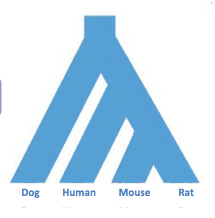
\includegraphics{\getdir/SpeciesTree.png}}
  \caption{Species Tree}
  \label{SpeciesTree}
\end{figure}

\subsection {Gene Tree}
Gene trees are trees that look at specific genes in different species (leaves are genes). The leaves of gene trees are labeled with gene sequences or gene ids associated with specific sequences. Figure~\ref{GeneTree} shows an example of a gene tree that has 4 genes (leaves). The sequences associated with each gene are presented on the right side of Figure~\ref{GeneTree}.
\begin{figure}[H]
  \centering
  \scalebox{.5}{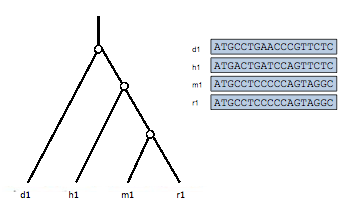
\includegraphics{\getdir/GeneTree.png}}
  \caption{Gene Tree}
  \label{GeneTree}
\end{figure}

\subsection{Gene Family Evolution}
Gene trees evolve inside a species tree.  An example of a gene tree contained in a species tree is shown in Figure~\ref{GeneSpecies} below.

\begin{figure}[H]
  \centering
  \scalebox{.4}{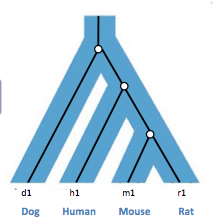
\includegraphics{\getdir/GeneSpecies.png}}
  \caption{Gene Tree Inside a Species Tree}
  \label{GeneSpecies}
\end{figure}
The next sub section explains how we can fit gene trees inside a species trees using Reconciliation.

\subsection{Reconciliation}

\noindent Reconciliation is an algorithm that helps compare gene trees to genome trees by fitting a gene tree fits inside a species tree. This is done by by mapping the vertices in the gene tree to vertices in the species tree. This sub section will focus on Reconciliation, related definitions, algorithm (Maximum Parsimony Reconciliation algorithm) and examples. 
\subsubsection{Definitions}
Two genes are {\bf orthologs} if their recent common ancestor (MRCA) is a speciation (splitting into different species).
\newline {\bf Paralogs} are genes whose MRCA is a duplication.
\newline Figure~\ref{Fig07_GeneFamilyEvolution} below illustrates how these types of genes can be represented in a gene tree. The tree below has 4 speciation nodes, one duplication and one loss.
 
\begin{figure}[H]
  \centering
  \scalebox{.25}{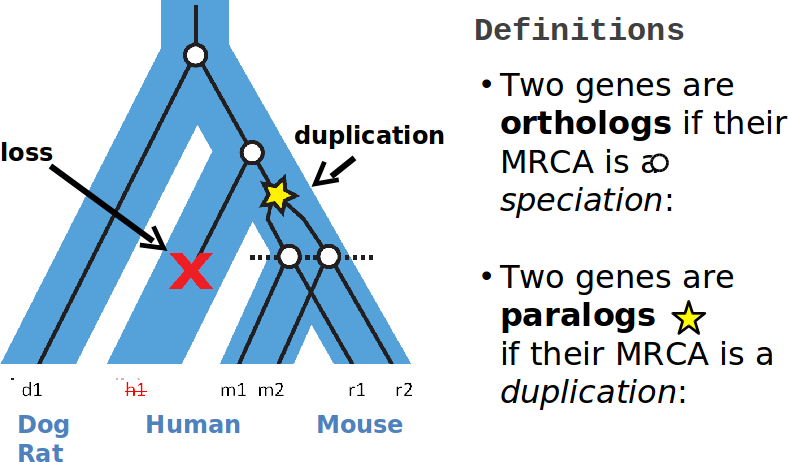
\includegraphics{\getdir/Fig07_GeneFamilyEvolution.png}}
  \caption{Gene Family Evolution: Gene Trees and Species Trees}
  \label{Fig07_GeneFamilyEvolution}
\end{figure}

A mapping diagram is a diagram that shows the node mapping from the gene tree to the species tree. Figure~\ref{MappingDiagram} shows an example of a mapping diagram.

\begin{figure}[H]
  \centering
  \scalebox{.4}{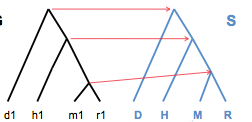
\includegraphics{\getdir/MappingDiagram.png}}
  \caption{Mapping Diagram}
  \label{MappingDiagram}
\end{figure}

A nesting diagram shows how the gene tree can be nested inside the species tree. For every mapping diagram there is a nesting diagram. Figure~\ref{NestingDiagram} shows an example of a possible nesting diagram for the mapping diagram in Figure~\ref{MappingDiagram}.
\begin{figure}[H]
  \centering
  \scalebox{.4}{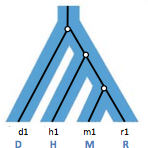
\includegraphics{\getdir/NestingDiagram.png}}
  \caption{Nesting Diagram}
  \label{NestingDiagram}
\end{figure}

\subsubsection{Maximum Parsimony Reconciliation (MPR) algorithm}
MPR is an algorithm that fits a gene tree in a species tree while minimizing the number of duplications and deletions.
\begin{figure}[H]
  \centering
  \scalebox{.3}{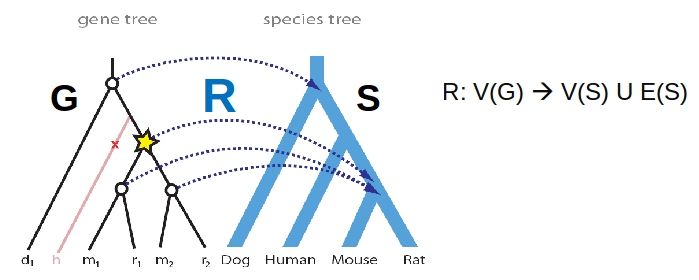
\includegraphics{\getdir/Fig08_MaximumParsimonyReconciliation.png}}
  \caption{Maximum Parsimony Reconciliation (MPR) } 
  \label{Fig08_MaximumParsimonyReconciliation}
\end{figure}

\noindent Given a gene tree and a species tree, the algorithm finds the reconciliation that minimizes the number of duplications and deletions. Figure~\ref{Fig08_MaximumParsimonyReconciliation} above shows an example of a possible mapping from a gene tree to a species tree. Figure~\ref{Fig09_MPRAlgorithm} presents the pseudocode for the MPR algorithm.

\begin{figure}[H]
  \centering
  \scalebox{.3}{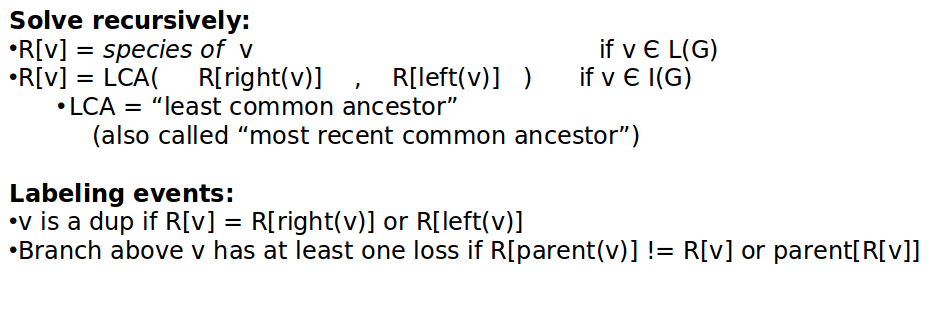
\includegraphics{\getdir/Fig09_MPRAlgorithm.png}}
  \caption{Maximum Parsimony Reconciliation Recursive Algorithm} 
  \label{Fig09_MPRAlgorithm}
\end{figure}

\noindent We map the arrows low as possible, since lower mapping usually results in fewer events. However, we cannot map too low. We map as low as we can without violating the descendent-ancestor relationships. The algorithm goes recursively from bottom up, starting from the leaves. We already know the mapping for the leaves, so we can easily map them. To map the ancestors, for each node (going recusively up the tree) we look at the right child and left child and take the least common ancestor (LCA) of the species that they map to. If a node maps to its right or left child, we know there is a duplication. An expected branch that does not exist indicates a loss.   
%\noindent Duplication events map to the same as both of its children. Loss event
%maps to gap in the mapping. Gene tree accuracy is important; even one
%branch misplaced can dramatically increase error.

\subsubsection{Reconciliation Examples}

\begin{figure}[H]
  \centering
  \scalebox{.5}{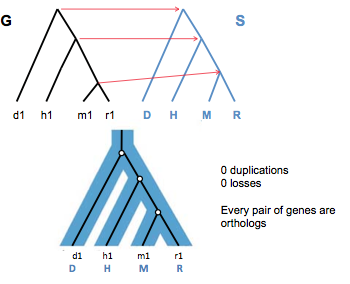
\includegraphics{\getdir/ReconciliationExample1.png}}
  \caption{Reconciliation Example 1, simple mapping case} 
  \label{ReconciliationExample1}
\end{figure}
In Figure~\ref{ReconciliationExample1}, the nodes can be mapped straight across, since there are no duplications or losses.

\begin{figure}[H]
  \centering
  \scalebox{.5}{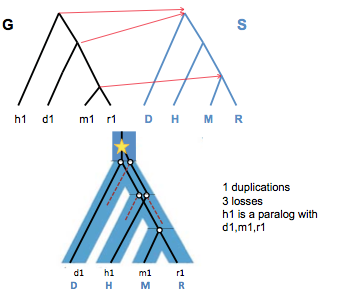
\includegraphics{\getdir/ReconciliationExample2.png}}
  \caption{Reconciliation Example 2, parsimonious reconciliation for complex case} 
  \label{ReconciliationExample2}
\end{figure}
\noindent In Figure~\ref{ReconciliationExample2}, we see a parsimonious (minimum number of losses and duplications) reconciliation for a case in which nodes from the gene tree cannot be mapped straight across.  

\begin{figure}[H]
  \centering
  \scalebox{.5}{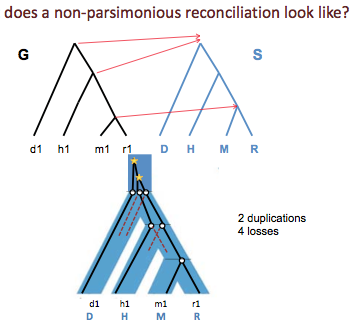
\includegraphics{\getdir/ReconciliationExample3.png}}
  \caption{Reconciliation Example 3, non parsimonious reconciliation for complex case} 
  \label{ReconciliationExample3}
\end{figure}
\noindent Figure~\ref{ReconciliationExample3} shows a non-parsimonious reconciliation . The parsimonious mapping for the same trees is shown in Figure~\ref{ReconciliationExample1}.

\begin{figure}[H]
  \centering
  \scalebox{.5}{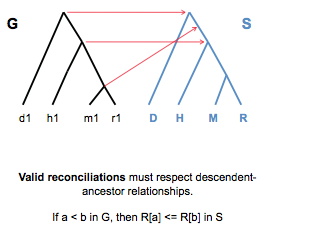
\includegraphics{\getdir/ReconciliationExample4.png}}
  \caption{Reconciliation Example 4, invalid Reconciliation} 
  \label{ReconciliationExample4}
\end{figure}
\noindent Figure~\ref{ReconciliationExample4}  shows an invalid reconciliation. This reconciliation is \underline{invalid} since it does not respect descendent-ancestor relationships. In order for this reconciliation to be possible, the descendent would have to travel back in time and be created before its ancestor. Clearly, such a scenario would be impossible. A valid reconciliation must satisfy the following: {\bf If a $<$ b in G, then R[a] $\le$ R[b] in S}.

\section{Reconstruction}
In the previous section we learned how  to compare gene trees and species trees. In this section, we will use this information to reconstruct gene trees and species trees. 

\subsection{Species Tree Reconstruction}
In the past, it was really hard to identify a marker gene for a specific species. As sequencing improved we started having lots of sequencing data, people started building trees for different loci. The tree you got highly dependent on the tree you used. Possible reasons why trees differ include noise (from statistical estimate errors and noise), hidden duplications and losses and allele sorting in a population.

\subsubsection{Species Tree Reconstruction Problem}

\begin{figure}[H]
  \centering
  \scalebox{.5}{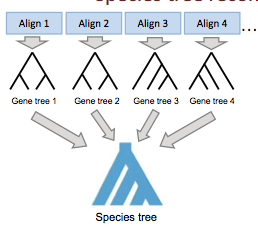
\includegraphics{\getdir/SpeciesTreeReconstruction.png}}
  \caption{Species Tree Reconstruction} 
  \label{SpeciesTreeReconstruction}
\end{figure}

Given lots of different gene trees that disagree, our goal is to make them into once species tree (as shown in Figure~\ref{SpeciesTreeReconstruction}. There are lots of different algorithms that reconstruct species trees. These algorithms include Supermatrix methods (Rokas 2003, Ciccareli 2006), Supertree methods (Creevey \& McInerney 2005), Minimizing Deep Coalescence (Maddison \& Knowles 2006) and  Modeling coalescence (Liu \& Pearl 2007). 

One way to do this, which is mostly effective for noisy data, is to
pull more data together in order to increase accuracy. This is done by concatenating gene alignments into a super-matrix.

Another method involves building a tree for each one and using a consensus method to summarize these trees. Then we identify branches that frequently across the trees and build a species tree that has the branches that occur most frequently.

There is another way to reconstruct a species tree, which is effective in case the gene trees disagree because of duplications and losses. The goal is to find the species tree that applies the fewest duplications. We build all the gene trees and then propose a species tree. Next, we use reconciliation to determine the number of events each gene tree combined with the proposed species tree implies. Then, we propose other species trees and move branches around. Wrong species trees tend to have lots of events that did not happen. The correct tree should have the fewest number of events. 


\subsection{Improving Gene Tree Reconstruction and Learning Across Gene Trees}
We can use methods similar to those described above to build better gene trees. This can be done by using information from a species tree to study a gene tree of interest. For example, species trees can be used to determine when losses and duplications occurred. The idea is that we can use the fact that species trees are often built from the entire genome, to obtain more information about related gene trees. We can use both the branch length and the number of events to do this. 

\begin{figure}[ht!]
  \centering
  \scalebox{.3}{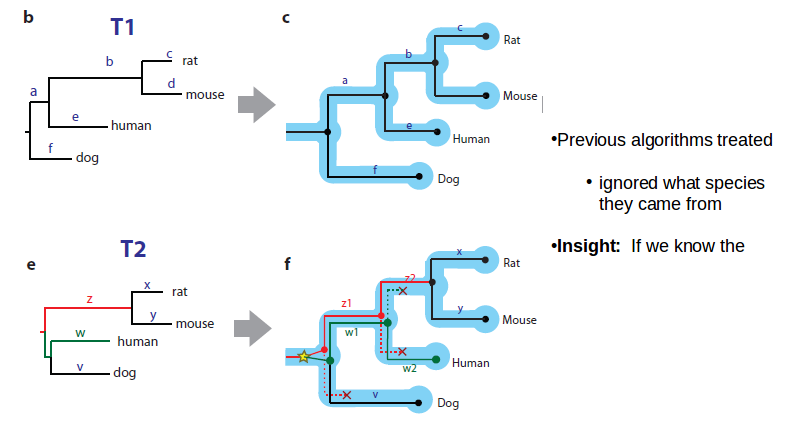
\includegraphics{\getdir/Fig10_LearningAcrossGeneTrees.png}}
  \caption{Using species trees to improve gene tree reconstruction.} 
  \label{Fig10_LearningAcrossGeneTrees}
\end{figure}

If we know the species tree, we can develop a model for what kind of
branch lengths we can expect. We can use conserved gene order to tell
orthologs and build trees.

\begin{figure}[ht!]
  \centering
  \scalebox{.3}{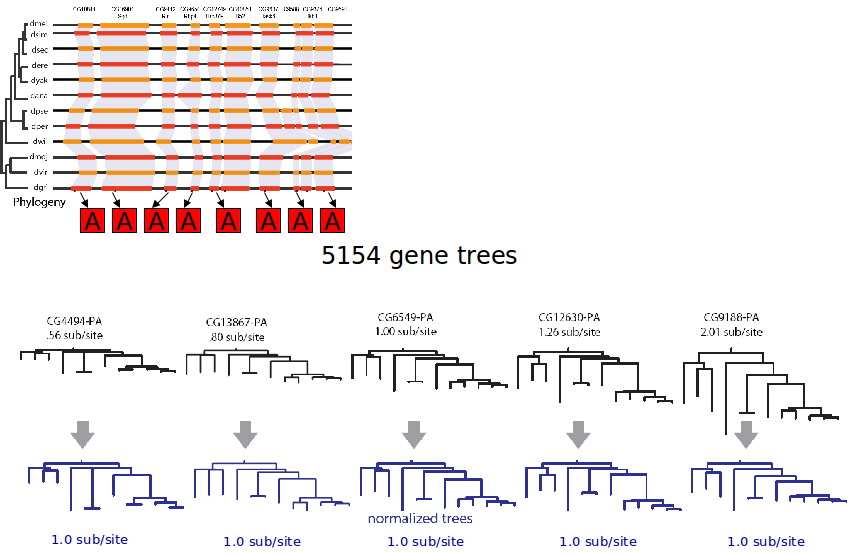
\includegraphics{\getdir/Fig11_DevelopingRatesModel.png}}
  \caption{We can develop a model for what kind of branch lengths we
    can expect. We can use conserved gene order to tell orthologs and
    build trees.}
  \label{Fig11_DevelopingRatesModel}
\end{figure}

When a gene is fast evolving in one species, it is fast evolving in all
species. We can model a branch length as two different rate
components. One is gene specific(present across all species) and the other is
species specific, which is customized to a specific species.

\begin{figure} [ht!] 
  \centering
  \scalebox{.3}{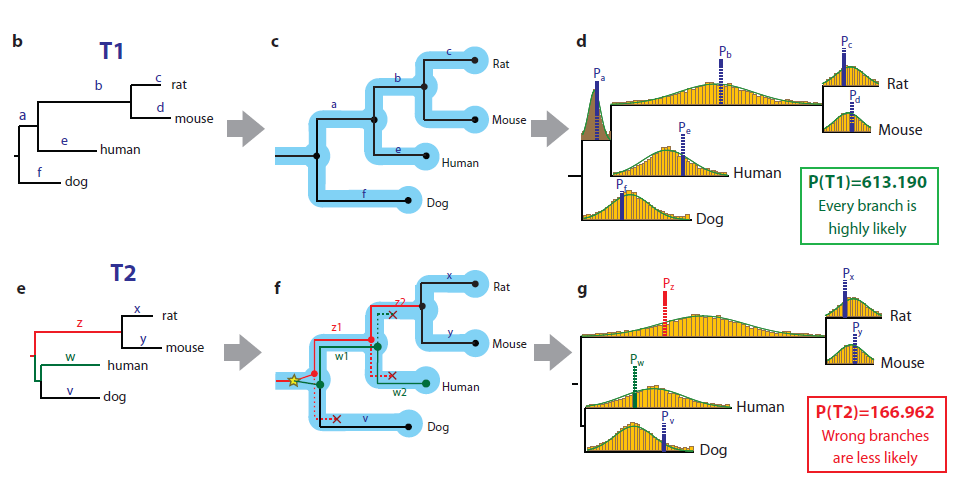
\includegraphics{\getdir/Fig12_UsingRateModels.png}}
  \caption{Branch length can be modeled as two different rate
    components: gene specific and species specific.}
  \label{Fig12_UsingRateModels}
\end{figure} 

\noindent This method greatly improves reconstruction accuracy.


\section{Modeling Population and Allele Frequencies}
With the advent of next-gen sequencing, it is becoming economical to
sequence the genomes of many individuals within a population. In order
to make sense of how alleles spread through a population, it's helpful
to have a model to compare data against. The \textbf{Wright-Fisher} 
reproduction model has filled this role for the past 70 years.

\subsection{The Wright-Fisher Model}

Like HMMs, Wright-Fisher is a Markov process: at each step, the system
randomly progresses, and the current state of the system depends only 
on the previous state. In this case, state transitions represent reproduction.
By modeling the transmission of chromosomes to offspring, we can study genetic drift.

The model makes a number of simplifying assumptions:
\begin{enumerate}
\item Population size, \textbf{N}, is constant at each generation.
\item Only members of the same generation reproduce (no overlap).
\item Reproduction occurs at random.
\item The gene being modeled only has 2 alleles.
\item Genes undergo neutral selection.
\end{enumerate}

\begin{figure} [ht!] 
  \centering 
  \scalebox{.3}{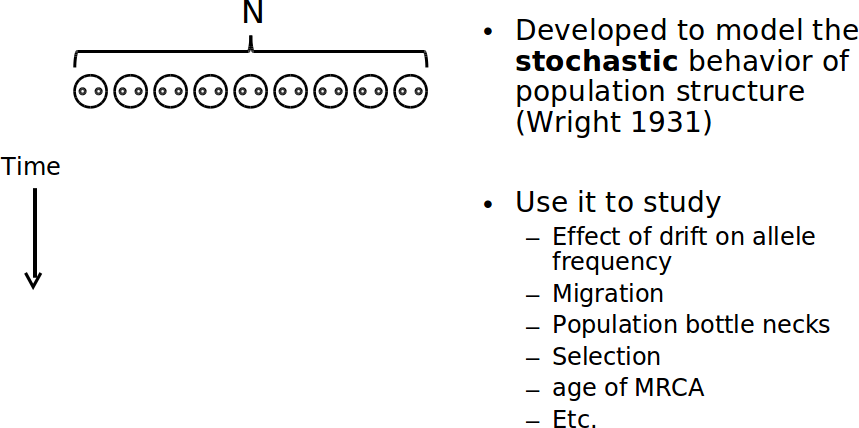
\includegraphics{\getdir/Fig13_FisherWrightModel.png}}
  \caption{The Wright-Fisher model}
  \label{Fig13_FisherWrightModel}
\end{figure}

Note that Wright-Fisher is not an appropriate choice if you're trying to
model the change in frequency of a gene that is positively or negatively
selected for. If we use Wright-Fisher to model the chromosomes of diploid
individuals, the population size of the model becomes \textbf{2N}.


In English, here's how Wright-Fisher works:

At every generation, for each child, we randomly select from the parents (with replaccement). The allele of the child becomes that of the randomly selected parent.

We repeat this process for many generation, with the children serving as the new parents, ignoring the ordering of chromosomes.


It really is that simple. To determine the probability of $k$ copies of an allele
existing in the child generation when it had a frequency of $p$ in the parent
generation, we can use this formula:

\begin{align}
\binom{2N}{k} p^{k} q^{2N-k}
\end{align}

Here, $q = (1-p)$. It is the frequency of non-p alleles in the parent generation.

\begin{figure} [h] 
  \centering 
  \scalebox{.3}{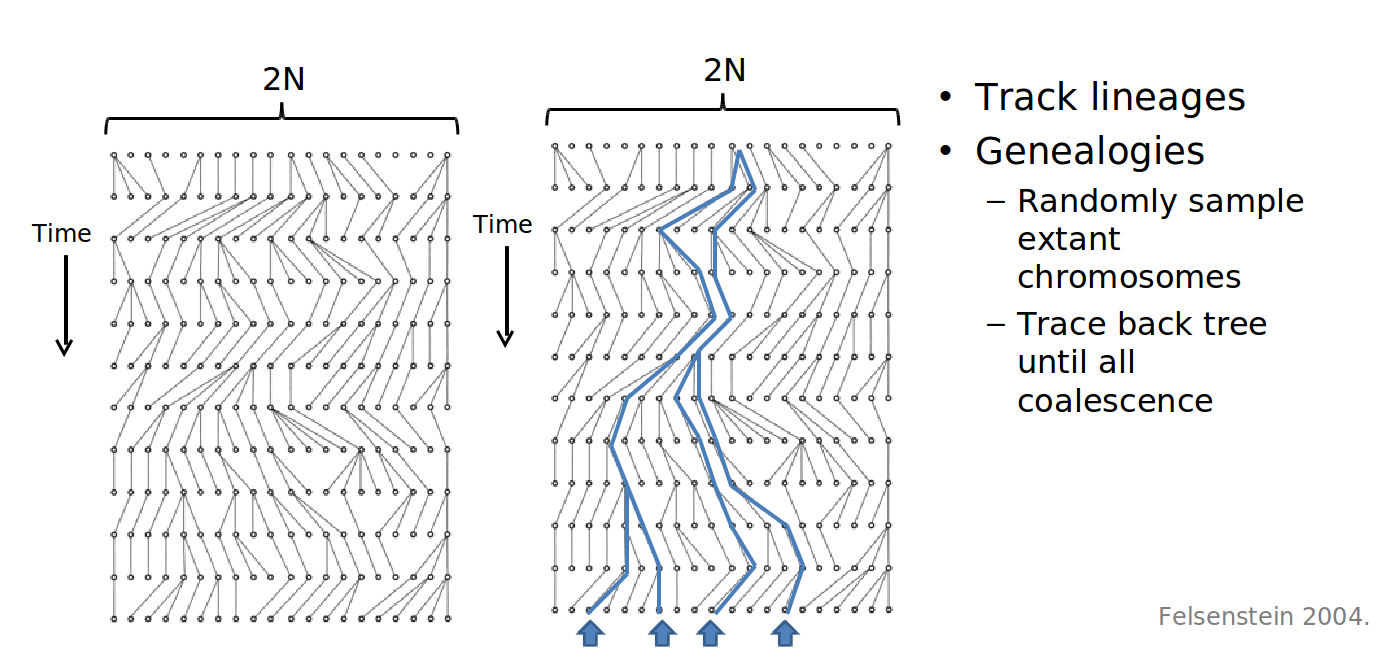
\includegraphics{\getdir/Fig14_FisherWrightManyGenerations.png}}
  \caption{Many iterations of Wright-Fisher yielding a lineage tree}
  \label{Fig14_FisherWrightManyGenerations}
\end{figure}

Now we can begin to explore such questions as: how probable is it and how many generations is it expected to take for a given allele to become \textbf{fixed}, meaning the allele is present in \textit{every} member of the population?

The expected time (in generations) for fixation, given the assumptions made by Wright-Fisher, is proportionate to $4N_{E}$, where $N_{E}$ is the effective population size.

Again, it's important to keep in mind the limitations of this model and ask if it actually makes sense for the system you're trying to represent. Consider how you could tweak the proposed model to account for a selection coefficient ranging between -1 (lethal negative selection) and 1 (strong positive selection).

\pagebreak
\subsection{The Coalescent Model}

The problem with the Wright-Fisher model is that it assumes you know the allele frequencies of the ancentral generation. When dealing with the genomes of present species, these quantities are unknown. The Coalescent Model solves this conundrum by thinking retrospectively. That is to say: we start with the alleles of the \textit{current} generation, and work our way \textit{backwards} in time. The basic Coalescence Model makes the same assumptions as Wright-Fisher. At each generation, we ask: what is the probability of the two identical alleles coalescing, or sharing a parent, in the previous generation.

We can pose the probability of a coalescence event occuring in the previous generation as the probability of coalescence \textit{not} occuring in any of the $t-1$ generations prior to the last one, times the probability of it occuring in the previous (the t-th) generation. This is equivalent to the expression:

\begin{align}
P_c(t) = \left(1-\frac{1}{2N_e}\right)^{t-1} \left(\frac{1}{2N_e}\right)
\end{align}

Where $N_e$ is the effective population size.

\begin{figure} [ht!] 
  \centering 
  \scalebox{.3}{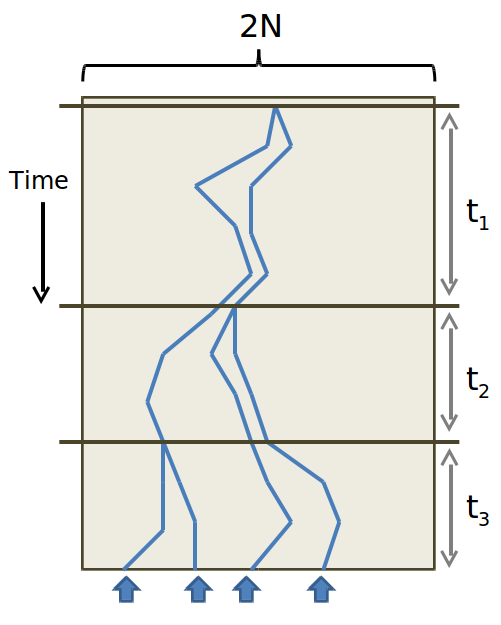
\includegraphics{\getdir/Fig15_CoalescentModel.png}}
  \caption{The coalescent model.}
  \label{Fig15_CoalescentModel}
\end{figure}

By approximating this geometric distribution as an exponential one: $ P_c(t) = \frac{1}{2N_e}e^{- \left( \frac{t-1}{2N_e} \right)}$, we can determine the expected number of generations back until coalescence, which turns out to be $2N_e$, with a standard deviation of $2N_e$.

To ask about the coalescence of \textit{multiple} lineages at a given generation, we must, as in Wright-Fisher, use a binomial distribution. The probability of $k$ lineages coalescing for the \textit{first} time at generation t is:

\begin{align}
  P(T_k = t) = \left( 1 - \binom{k}{2} \frac{1}{2N} \right)^{t-1} \binom{k}{2} \frac{1}{2N}
\end{align}
 
And again, this can be approximated with an exponential distribution for sufficiently large k. The individual at which two lineages converge is referred to as the \textbf{Most Recent Common Ancestor}. By continually moving backwards until all ancestors coalesce, we end up with a new kind of tree! And by comparing the tree resulting from coalescence with a gene tree we've constructed, discrepancies between the two may signal that certain assumptions of the Coalescent Model have been violated. Namely, selection may be occuring.

\begin{figure} [ht!] 
  \centering 
  \scalebox{.3}{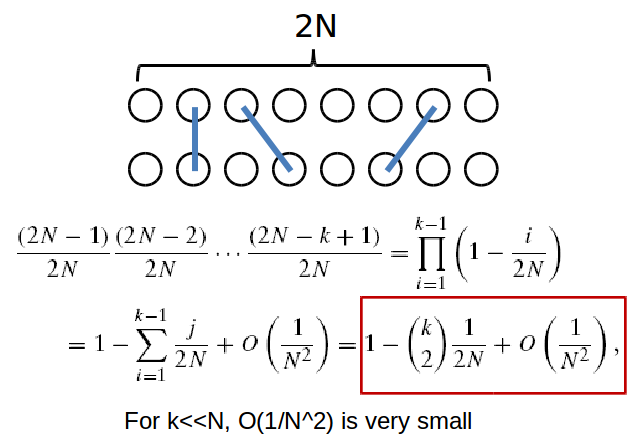
\includegraphics{\getdir/Fig16_CoalescentProbDist.png}}
  \caption{Geometric probability distribution for coalescent events in k lineages.}
  \label{Fig16_CoalescentProbDist}
\end{figure} 

\pagebreak
\subsection{The Multispecies Coalescent Model}

\begin{figure} [ht!] 
  \centering 
  \scalebox{.3}{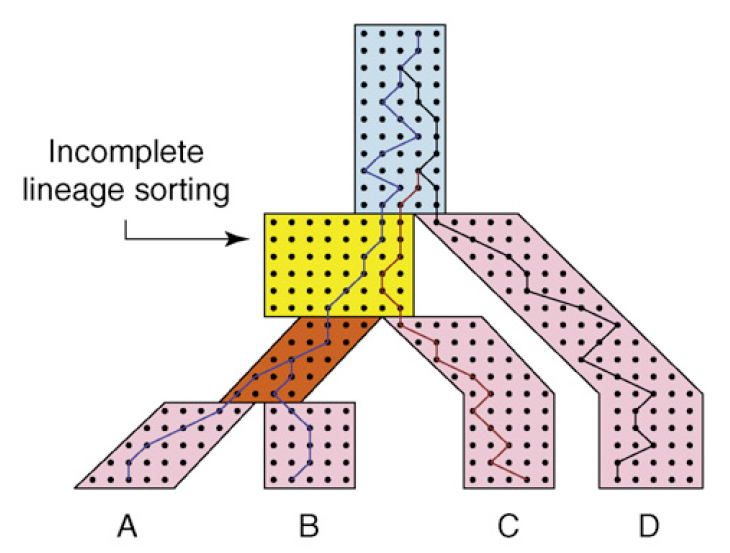
\includegraphics{\getdir/Fig17_MultispeciesCoalescent.png}}
  \caption{Multispecies Coalescent Model.}
  \label{Fig17_MultispeciesCoalescent}
\end{figure}

We can take this idea once step further and track coalescence events 
across multiple species. Here, each genome of an individual species is treated as a lineage.

Note that there is a lag time between the separation of two populations and 
the time at which two gene lineages coalesce into a common ancestor.
Also note how the rate of coalescence slows down as N gets bigger and for short branches.

In the image above, deep coalescence is depicted in light blue for three 
lineages. The species and gene trees here are incongruent since 
C and D are sisters in gene tree but not the species tree.

There is a $\frac{2}{3}$ chance that incongruence 
will occur because once we get to the light blue section, Wright-Fisher
is memoryless and there is only $\frac{1}{3}$ chance that it will be
congruent. The effect of incongruence is called \textbf{Incomplete Lineage Sorting}. By measuring the frequency at which \textbf{ILS} occurs, we gain insight into unusually large populations or unsually short branch lengths within the species tree.

You can build a maximum parsimony species tree based on the notion of minimizing the number of ILS events rather than minimizing implied duplication/loss events as covered previously. It is even possible to combine these two methods to, ideally, create a phylogeny that is more accurate than either of them would be individually.

\section{SPIDIR:Background} 
As presented in the supplementary information for SPIDIR, a gene
family is the set of genes that are descendents of a single gene in
the most recent common ancestor (MRCA) of all species under
consideration. Furthermore, genetic sequences undergo evolution at
multiple scales, namely at the level of base pairs, and at the level
of genes. In the context of this lecture, two genes are orthologs if
their MRCA is a speciation event; two genes are paralogs if their MRCA
is a duplication event.

In the genomic era, the species of a modern genes is often known;
ancestral genes can be inferred by reconciling gene- and
species-trees. A reconciliation maps every gene-tree node to a
species-tree node. A common technique is to perform Maximum Parsimony
Reconciliation (MPR), which finds the reconciliation R implying the
fewest number of duplications or losses using the recursion over inner
nodes $v$ of a gene tree $G$. MPR fist maps each leaf of the gene tree
to the corresponding species leaf of the species tree. Then the
internal nodes of $G$ are mapped recursively:

$R(v) = MRCA(R(right(v)),R(left(v)))$

\noindent If a speciation event and its ancestral node are mapped to the same node on the species tree. Then the ancestral node must be an duplication event.

Using MPR, the accuracy of the gene tree is crucial. Suboptimal gene
trees may lead to an excess of loss and duplication events. For
example, if just one branch is misplaced (as in
\ref{Fig02_MLScoringStep}) then reconciliation infers 3 losses and 1
duplication event. In \cite{Rasmussen}, the authors show that the
contemporaneous current gene tree methods perform poorly (60\%
accuracy) on single genes. But if we have longer concatenated genes,
then accuracy may go up towards 100\%. Furthermore, very quickly or
slowly evolving genes carry less information as compared with
moderately diverging sequences (40-50\% sequence identity), and
perform correspondingly worse. As corroborated by simulations, single
genes lack sufficient information to reproduce the correct species
tree. Average genes are too short and contains too few
phylogenetically informative characters. While many early gene tree
construction algorithms ignored species information, algorithms like
SPIDIR capitalize on the insight that the species tree can provide
additional information which can be leveraged for gene tree
construction. Synteny can be used to independently test the relative
accuracy of different gene tree reconstructions. This is because
syntenic blocks are regions of the genome where recently diverged
organisms have the same gene order, and contain much more information
than single genes.

\begin{figure} [ht!] 
  \centering 
  \scalebox{.3}{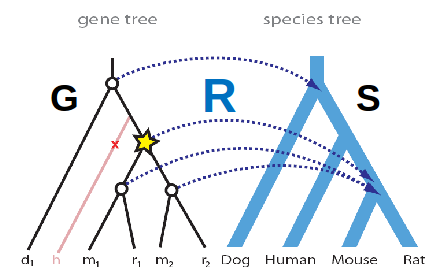
\includegraphics{\getdir/Fig18_AlternateReconciliations.png}}
  \caption{MPR reconciliation of genes and species tree.}
  \label{Fig18_AlternateReconciliations}
\end{figure} 

\begin{figure} [ht!] 
  \centering 
  \scalebox{.3}{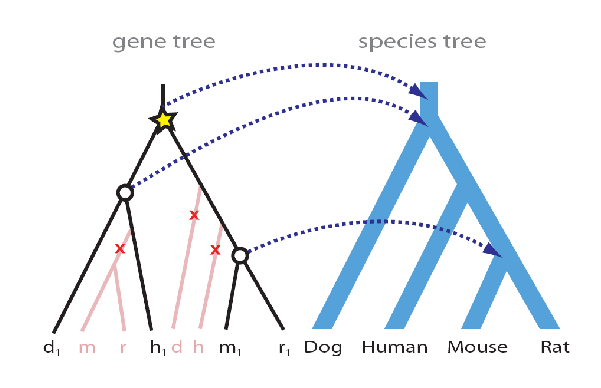
\includegraphics{\getdir/Fig19_GeneTreeInaccuracies.png}}
  \caption{Inaccuracies in gene tree.}
  \label{Fig19_GeneTreeInaccuracies}
\end{figure} 

There have been a number of recent phylogenomic algorithms including:
RIO \cite{Zmasek}, which uses neighbor joining (NJ) and bootstrapping
to deal with incogruencies, Orthostrapper \cite{Storm}, which uses NJ
and reconciles to a vague species tree, TreeFAM \cite{Li}, which uses
human curation of gene trees as well as many others. A number of
algorithms take a more similar track to SPIDIR \cite{Rasmussen},
including \cite{Arvestad}, a probabilistic reconciliation algorithm
\cite{Hollich}, a Bayesian method with a clock,\cite{Wapinski},and
parsimony method using species tree , as well as more recent
developments: \cite{Akerborg} a Bayesian method with relaxed clock and
\cite{Rasmussen2011}, a Bayesian method with gene and species specific
relaxed rates (an extension to SPIDIR) .

\section{SPIDIR: Method and Model} 
SPIDIR exemplifies an iterative algorithm for gene tree construction
using the species tree. In SPIDIR, the authors define a generative
model for gene-tree evolution. This consists of a prior for gene-tree
topology and branch lengths. SPIDIR uses a birth and death process to
model duplications and losses (which informs the prior on topology)
and then then learns gene-specific and species-specific substitution
rates (which inform the prior on branch lengths). SPIDIR is a
\textit{Maximum a posteriori (MAP)} method, and, as such, enjoys
several nice optimality criteria.

In terms of the estimation problem, the full SPIDIR model appears as
follows:

$argmax L,T,R P(L,T,R|D,S,\Theta) = argmax L,T,R P(D|T,L)P(L|T,R,S,\Theta)P(T,R|S,\Theta)$ 

The parameters in the above equation are: $D$ = alignment data , $L$ =
branch length $T$ = gene tree topology , $R$ = reconciliation , $S$ =
species tree (expressed in times) , $\Theta$ = ( gene and species
specific parameters [estimated using EM training], $\lambda$, $\mu$
dup/loss parameters)). This model can be understood through the three
terms in the right hand expression, namely:

\begin{enumerate} 
\item the sequence model-- $P(D|T,L)$. The authors used the common HKY
  model for sequence substitutions, which unifies Kimura's two
  parameter model for transitions and transversions with Felsenstein's
  model where substitution rate depends upon nucleotide equilibrium
  frequency.
\item the first prior term, for the rates model-- $P(L|T,R,S,\Theta)$,
  which the authors compute numerically after learning species and
  gene specific rates.
\item the second prior term, for the duplication/loss model--
  $P(T,R|S,\Theta)$, which the authors describe using a birth and
  death process.
\end{enumerate} 

Having a rates model is very rates model very useful, since mutation
rates are quite variable across genes. In the lecture, we saw how
rates were well described by a decomposition into gene and species
specific rates. In lecture we saw that an inverse gamma distribution
appears to parametrize the gene specific substitution rates, and we
were told that a gamma distribution apparently captures species
specific substitution rates. Accounting for gene and species specific
rates allows SPIDIR to build gene trees more accurately than previous
methods. A training set for learning rate parameters can be chosen
from gene trees which are congruent to the species tree. An important
algorithmic concern for gene tree reconstructions is devising a fast
tree search method. In lecture, we saw how the tree search could be
sped up by only computing the full $argmax L,T,R P(L,T,R|D,S,\Theta)$
for trees with high prior probabilites. This is accomplished through a
computational pipeline where in each iteration 100s of trees are
proposed by some heuristic. The topology prior $P(T,R|D,S,\Theta)$ can
be computed quickly. This is used as a filter where only the
topologies with high prior probabilities are selected as candidates
for the full likelihood computation.

\noindent The performance of SPIDIR was tested on a real dataset of 21
fungi. SPIDER recovered over 96\% of the synteny orthologs while other
algorithms found less than 65\%. As a result, SPIDER invoked much
fewer number of duplications and losses.

\section{Ancestral Recombination Graphs}

\todo[Next Year]{Song, Yuns}{Fill in this section based on: www.eecs.berkeley.edu/~yss/Pub/SH-JCB05.pdf and the course notes from 2012.}

\subsection{The Sequentially Markov Coalescent}

\todo[Next Year]{Song, Yuns}{Fill this in based on: http://www.ncbi.nlm.nih.gov/pubmed/21270390}

\section{Conclusion} 
Incorporating species tree information into the gene tree building
process via introducing separate gene and species substitution rates
allows for accurate parsimonious gene tree reconstructions. Previous
gene tree reconstructions probably vastly overestimated the number of
duplication and loss events. Reconstructing gene trees for large
families remains a challenging problem.

\section{Current Research Directions}
\section{Further Reading}
\section{Tools and Techniques} 
\section{What Have We Learned?}

\nocite{*}
\bibliographystyle{plain}
\bibliography{Lecture21_Phylogenomics} 
